\documentclass[12pt, a4paper]{article}
% \documentclass[8pt, a4paper, twocolumn]{article}

\usepackage{amsmath}
\usepackage{amssymb}
\usepackage{amsthm}
\usepackage[utf8]{inputenc}
\usepackage[english]{babel}
\usepackage{indentfirst}
\usepackage{graphicx}
\usepackage{mathtext}
\usepackage[T1,T2A]{fontenc}
\usepackage{listings}
\usepackage{hyperref}
\usepackage{stmaryrd}
\usepackage{a4wide}
\usepackage{pgfplots}
\usepackage{tikz}
\usepackage{subcaption}
\usepackage{mathtools}

\lstset{basicstyle=\ttfamily\footnotesize,breaklines=true}
\definecolor{darkGreen}{RGB}{31, 140, 47}
\definecolor{darkBlue}{RGB}{31, 53, 125}
\definecolor{brightYellow}{RGB}{245, 210, 10}   
\title{\text{Additive drift with tail bounds}}

% \date{04-08-2021}

\newcommand\setItemnumber[1]{\setcounter{enumi}{\numexpr#1-1\relax}}
\DeclareMathOperator*{\argmin}{arg\,min}

\newcommand{\gfun}{\mathbf{g}}
\newcommand{\Lim}[1]{\raisebox{0.5ex}{\scalebox{0.8}{$\displaystyle \lim_{#1}\;$}}}


\newcounter{casenum}
\newenvironment{caseof}{\setcounter{casenum}{1}}{\vskip.5\baselineskip}
\newcommand{\case}[2]{\vskip.5\baselineskip\par\noindent {\bfseries Case \arabic{casenum}:} #1\\#2\addtocounter{casenum}{1}}

\newtheorem{theorem}{Theorem}[section]
\newtheorem{corollary}{Corollary}[theorem]
\newtheorem{lemma}[theorem]{Lemma}
\theoremstyle{remark}
\newtheorem*{remark}{Remark}
\theoremstyle{definition}
\newtheorem*{exmp}{Example}

\newcommand{\expx}[1]{e^{-|x|^{#1}}}
\newcommand{\expxpoz}[1]{e^{-x^{#1}}}
\newcommand{\infint}[1]{\int_{-\infty}^{+\infty} #1 \, dx}
\newcommand{\infintpoz}[1]{\int_{0}^{+\infty} #1 \, dx}
\newcommand{\der}[2]{\frac{\partial #1}{\partial #2}}
\newcommand{\cm}{coming soon\dots}
\newcommand{\expp}[1]{E[e^{#1 \Delta_t}]}
\newcommand{\limd}{\lim\limits_{d \to +\infty}}

\newcommand{\underrel}[2]{\mathrel{\mathop{#2}\limits_{#1}}}

% Denis's commands

\newcommand{\N}{{\mathbb N}}
\newcommand{\R}{{\mathbb R}}
\newcommand{\eps}{\varepsilon} 

\newcommand{\todo}[1]{\textbf{\textcolor{red}{TODO: #1}}}

\DeclareMathOperator{\Geom}{Geom}

\author{Vihnin F.
    \and Antipov D.
    \and Sinyachenko N.}


\begin{document}
\maketitle

\section{Introduction}

Drift analysis is a powerful toolbox for the analysis of random processes. Taking the roots from Hajek's negative drift~\cite{Hajek82} drift analysis was significantly developed by the evolutionary computation community starting with a seminal work by He and Yao~\cite{HeY04} introducing the additive drift theorem. Since then many modifications have been produced such as multiplicative drift~\cite{DoerrJW12} and variable drift~\cite{Johannsen10,RoweS12}. The most recent overview of the family of drift theorems can be found in~\cite{Lengler17}.

All drift theorems consider a random process $\{X_t\}_{t \in \N}$, which starts with some $X_0 = a$ and aims to reach some value $b$. \todo{Adapt all theorems to this notation or change the notation, if it is easier.} Without loss of generality, we assume that $a < b$\footnote{Some of the drift theorems are formulated for a process which starts at a greater value $b$ and aims to reach a smaller value $a$. However, such results can be inverted by considering a process $Y_t = -X_t$.}. The \emph{hitting time} $T$ for such process is the minimum $t$ such that $X_t \ge b$. The main idea of drift analysis is to transform the available information about the process such as the expected step size $E[X_{t + 1} - X_t \mid X_t = s]$ (which is called the \emph{drift} of the process) into information about the hitting time. E.g., the additive drift theorem claims that if the expected step size is bounded from below by some $\delta > 0$, then the expected hitting time is at most the distance $(b - a)$ which the process has to cover divided by $\delta$ (with some additional conditions such as $X_t$ cannot jump over its goal, that is, $X_t \le b$ for all $t \in \N$). More formally, we have
\begin{align*}
    E[T] \le \frac{b - a}{\delta}.
\end{align*}
The additive drift theorem also works into an opposite direction. That is, if the drift is bounded from above by some $\delta > 0$, then we have
\begin{align*}
    E[T] \ge \frac{b - a}{\delta}.
\end{align*}

Several other drift theorems are capable to give us more information about the hitting time. In particular, the multiplicative drift theorem~\cite{DoerrJW12} gives an exponentially small bound on the probability of the hitting time to exceed its expectation. The reason why the additive drift theorem does not give us any similar bounds on the concentration of the hitting time is that it uses only a small piece of information about the considered process, which is, the expected progress. To be able to obtain some tail bounds on the hitting time we should also have some bounds on the concentration of the steps of the process. For example, consider two processes $\{X_t\}_{t \in \N}$ and $\{Y_t\}_{t \in \N}$ which start with $X_0 = Y_0 = 0$ and the hitting time for these processes is when they reach $100$. Let $\{X_t\}_{t \in \N}$ be a deterministic process such that for all $t \in N$ we have $X_{t + 1} = X_t + 1$. Let $\{Y_t\}_{t \in \N}$ be a process such that with probability $\frac{1}{100}$ we have $Y_{t + 1} = Y_t + 100$ and we have $Y_{t + 1} = Y_t$ otherwise. Both processes have the same drift equal to one, and both processes reach $100$ in the same expected time, namely in 100 steps. However, the hitting time of $\{X_t\}_{t \in \N}$ is determined and has zero variation, while the hitting time of $\{Y_t\}_{t \in \N}$ follows a geometric distribution $\Geom(\frac{1}{100})$ and its standard deviation is $10\sqrt{99} \approx 99$.

In practice we often meet something in the middle between these two processes, namely processes with non-deterministic, but well-concentrated steps. Intuition suggests that for such processes the variation of the hitting time should not be large too. We are aware of two approaches for the analysis of such processes, which are, the analysis via sub-Gaussian processes shown in~\cite{Kotzing16} and the analysis via the negative drift theorem shown in~\cite{AntipovDK19}. We discuss both approaches and show that they have the same nature, however, they have different conditions when they are applicable. \todo{State exact results here: the differences and similarities.}

\section{Existing tools}

The two approaches for deriving the tail bounds on the hitting time for the processes under additive drift shown in~\cite{Kotzing16} and in~\cite{AntipovDK19} use the same trick. They decompose the random process $X_t$ into a sum of a deterministic process and a super- or sub-martingale. Namely, they consider
\begin{align*}
    X_t = Y_t + \eps t,
\end{align*}
where $\eps$ is a constant chosen in such a way that $Y_t$ is either za super- or sub-martingale.

When we aim at showing the lower tail bound, that is, for some time bound $B$ we want to estimate $\Pr[T \le B]$, then we must
\begin{enumerate}
    \item know the \emph{upper} bound $\delta$ on the expected progress of $X_t$ and
    \item choose $\eps$ which is at least $\delta$ so that $Y_t$ was a super-martingale.
\end{enumerate}
After that the main goal is to show that $Y_t$ does not exceed some value $c > 0$ in at least $B$ steps, since it would imply that $X_t$ does not exceed $\eps t + c$. Hence, if we consider only $B$ such that $(b - a) > \eps B + c$  then we have 
\begin{align*}
    \Pr[T \le B] = \Pr[\forall t \in[1..B] \  X_t < b] = \Pr[\forall t \in[1..B] \  Y_t < c].
\end{align*}
Note that this works only for $B < \frac{b - a - c}{\eps}$, which is less than the expected hitting time, since by the additive drift theorem we have
\begin{align*}
    E[T] \ge \frac{b - a}{\delta} > \frac{b - a - c}{\eps}.
\end{align*}

The main difference between the methods shown in~\cite{Kotzing16} and~\cite{AntipovDK19} is in how they estimate $\Pr[\forall t \in[1..B] \  Y_t < c]$. In~\cite{Kotzing16} we consider $Y_t$ which are sub-Gaussian processes and estimate the probability that they do not exceed $c$ using some tools specific for the sub-Gaussian processes. In~\cite{AntipovDK19} we consider $Y_t$ which are a subject to the Hajek's negative drift theorem. 

We describe these two approaches in more details in this section.

We also note that we can obtain the upper tail bounds (that is, estimates on the probability $\Pr[T > B]$) with similar arguments. For this we also need to use a decomposition $X_t = Y_t + \eps t$, but now we require
\begin{enumerate}
    \item the expected progress to be bounded from below by some $\delta > 0$ and
    \item $Y_t$ to be a sub-martingale.
\end{enumerate}  

\subsection{Negative drift}

In this section we discuss the Hajek's negative drift theorem, which is most commonly used in the following form.

\begin{theorem}[Drift Theorem for Lower Bounds] \label{thm:neat}
    Let $\{X_t\}_{t \ge 0}$ be a Markow process over a finite set of states $\mathbb{S}$, and $\mathbf{g} : \mathbb{S} \rightarrow \mathbb{R}$ a function that assigns to every state a non-negative real numbers. Let $a$ and $b$ be some real numbers such that $a < b$ and let the random variable $T$ denote
    the earliest point in time $t$ when $\mathbf{g}(X_t) \leq a$ holds.

    If there are constants $\lambda > 0$, $D \ge 1$, and $p > 1$ such that the following three conditions hold
    \renewcommand\labelenumi{(\theenumi)}
    \begin{enumerate}
        \item $\gfun(X_0) \ge b$,
        \item for all \(t \geq 0\) $ E\left[e^{-\lambda(\gfun(X_{t + 1}) - \gfun(X_t))} \Big|\ X_t,\ \gfun(X_t) < b\right] \leq 1 - \frac{1}{p} =: \rho$ and
        \item for all \(t \geq 0\) $ E\left[e^{-\lambda(\gfun(X_{t + 1}) - b)} \Big|\ X_t,\ \gfun(X_t) \ge b\right] \leq D$,
    \end{enumerate}
    then for all time bounds $B \ge 0$ the probability that $T$ exceeds $B$ is at most

    \begin{equation}
        \Pr[T \leq B] \leq e^{\lambda(a - b)} \cdot B \cdot D \cdot p
    \end{equation}
\end{theorem}

This form of the theorem is not stated in~\cite{Hajek82} and we are not aware of any proof which derives it from the results of Hajek's paper. Hence we present a simple proof of the negative drift theorem which is based on the following lemma from~\cite{Hajek82}.

\begin{lemma}[Lemma 2.8 in \cite{Hajek82}] \label{lm:haj}
    If conditions 2 and 3 are met then for all $t \geq 0$ we have

    $$\Pr[\gfun(X_t) \leq a] \leq \rho^te^{\lambda(a - \gfun(X_0))} + \frac{1 - \rho^t}{1 - \rho} D e^{\lambda(a - b)}$$

\end{lemma}

\begin{proof}[Proof of Theorem \ref{thm:neat}]

    If $T = B$, then we have $\gfun(X_k) \leq a$ and for all $t < B$ we have $\gfun(X_t) > a$. Hence, we compute

    \begin{align*}
        \Pr[T \leq B] & = \sum_{k=1}^{B} \Pr[T = k]                                                                        \\
                      & = \sum_{k=1}^{B} \Pr[\gfun(X_k) \leq a \land \gfun(X_{k - 1}) > a \land ... \land \gfun(X_0) > a)] \\
                      & \leq \sum_{k=1}^{B} \Pr[\gfun(X_k) \leq a].
    \end{align*}

    By Lemma $\ref{lm:haj}$

    \begin{align*}
        \Pr[T \leq B] & \leq \sum_{k=1}^{B} \left(\rho^k e^{\lambda(a - \gfun(X_0))} + \frac{1 - \rho^k}{1 - \rho} D e^{\lambda(a - b)}\right)                                                          \\
                      & = \rho \left(\frac{1 - \rho^B}{1 - \rho}\right) e^{\lambda a}\left(e^{-\lambda\gfun(X_0)} - \frac{D}{1 - \rho} e^{-\lambda b}\right) + e^{\lambda(a - b)} \frac{B D}{1 - \rho}.
    \end{align*}

    Since $\gfun(X_0) \ge b$ we have

    \begin{align*}
        \Pr[T \leq B] & \leq \rho \frac{1 - \rho^B}{1 - \rho} e^{\lambda (a - b)}\left(1 - \frac{D}{1 - \rho}\right) + e^{\lambda(a - b)} \frac{B D}{1 - \rho}
    \end{align*}

    Since $\frac{D}{1 - \rho} \geq D \geq 1 $, we further compute
    \begin{align*}
        \Pr[T \leq B] \leq e^{\lambda(a - b)} \frac{B D}{1 - \rho} = e^{\lambda(a - b)} \cdot B \cdot D \cdot p
    \end{align*}

\end{proof}
\subsection{Sub-Gaussian processes}

In~\cite{Kotzing16} the authors use the notion of sub-Gaussian processes, which are (informally speaking) the processes such that their steps are dominated by a normal distribution. More formally, a process $\{X_t\}_{t\in\N}$ is called $((c_t)_{t \in \N}, \delta)$-sub-Gaussian, iff for all $t \in \N$ and for all $\lambda \in [0, \delta]$ we have
\begin{align*}
    E\left[e^{\lambda(X_{t + 1} - X_t)} \mid X_1, \dots X_t\right] \le e^{z^2c_t/2}.
\end{align*}
If $c_t$ is equal to some $c$ for all $t \in \N$, then the process is called $(c, \delta)$-sub-Gaussian.
As it was noted in~\cite{Kotzing16}, all sub-Gaussian processes are super-martingales, that is, for all $t \in \N$ we have
\begin{align*}
    E[X_{t + 1} - X_t \mid X_1, \dots, X_t] \le 0.
\end{align*}

For such processes we have the following theorem (we slightly change the formulation in order to compare it with the negative drift approach).

\begin{theorem}[Theorem 11 in~\cite{Kotzing16}]
    Let $\{X_t\}_{t \in \N}$ be $((c_t)_{t \in \N}, \delta)$-sub-Gaussian. For all $t \in \N$ let $C_t \coloneqq \sum_{i = 1}^{t - 1} c_i$. Let $x>0$ be some constant and let $T$ be the minimum $t$ such that when $X_t \ge X_0 + x$. Then for all time bounds $B \in \N$ we have
    \begin{align*}
        \Pr\left[T \le B\right] \le \exp\left(-\frac{x}{2}\min\left\{\delta, \frac{x}{C_B}\right\}\right).
    \end{align*}
\end{theorem}


% \begin{theorem}
%     Suppose $X_t$ has a drift of at most $\varepsilon > 0$ and $(X_t - \varepsilon t)$ is $(c, \delta)$ - sub-Gaussian. Let \(X_0\) be \(a \in \mathbb{R}\) and let \(T\) be the first moment in time when \(X_t\) exceeds some \(b > a\). Then for all \(s \leq \frac{b - a}{2\varepsilon}\) we have

%     \[\Pr[T \leq s] \leq exp\left(-\frac{b - a}{4} min\left(\delta, \frac{b - a}{2cs}\right)\right)\]
% \end{theorem}

\subsection{Comparing requirements}
\label{sec:compare}
% To use some versions of drift theorems, we need some requirements on the sequence of random variables to be satisfied, such as the following:
% $$
%     \exists \delta \geq 0,\ c \in \mathbb{R} \ \forall  t \geq 0 \ \forall \gamma \in [0, \delta] $$$$
%     E\left[e^{\gamma (X_{t + 1} - X_{t})}\right] \leq e^{\frac{c \gamma^2}{2}},$$

% оr

% $$\exists \delta \geq 0,\ p \geq 1 \ \forall t \geq 0 $$$$
%     E\left[e^{\gamma (X_{t + 1} - X_{t})}\right] \leq 1 - \frac{1}{p}\ .$$

The theorem for sub-Gaussian processes is applicable, when there exist $\delta \geq 0$ and $c \in \mathbb{R}$ such that for all $t \geq 0$ and for all $\gamma \in [0, \delta]$ we have

$$  E\left[e^{\gamma (X_{t + 1} - X_{t})}\right] \leq e^{\frac{c \gamma^2}{2}}.$$

At the same time the negative drift theorem is applicable when there exist $\delta \geq 0$ and $p \geq 1$ such that for all $t \geq 0$ we have

$$
    E\left[e^{\gamma (X_{t + 1} - X_{t})}\right] \leq 1 - \frac{1}{p}\ .$$

To compare rigors of requirements we need to explore behavior of $E[e^{\gamma X}]$ depending to $\gamma$. This behavior depends on the distribution $X$, hence we consider the two cases for continuos and for discrete distributions.

\subsubsection*{Continuos distribution}

By the definition of the expectation of a function we have
\[
    E[e^{\gamma X}] = \int_{-\infty}^{+\infty} f(x) e^{\gamma x} \,dx,
\]

where $f(x)$ is a probability density function for $X$.

\hfill

Since we assume thet the integral is converging, compute the first derivative of this expectation over $\gamma$

\begin{align*}
    \frac{\partial E[e^{\gamma X}]}{\partial \gamma} & = \frac{\partial}{\partial \gamma} \int_{-\infty}^{+\infty} f(x) e^{\gamma x} \, dx = \int_{-\infty}^{+\infty} f(x) \frac{\partial e^{\gamma x}}{\partial \gamma} \, dx = \int_{-\infty}^{+\infty} x f(x) e^{\gamma x} \, dx = \\
    & = \int_{-\infty}^{0} x f(x) e^{\gamma x} \, dx + \int_{0}^{+\infty} x f(x) e^{\gamma x} \, dx.
\end{align*}

Note that for all $x \leq 0$ we have $e^{\gamma x} \leq 1$ and for all $x \geq 0$ we have $e^{\gamma x} \geq 1 + \gamma x$. Hence since $f(x) \geq 0$ for all x, we have

\begin{align*}
    \int_{0}^{+\infty} x f(x) e^{\gamma x} \, dx & \geq \int_{0}^{+\infty} x f(x) (1 + \gamma x)\, dx \\
    \int_{-\infty}^{0} x f(x) e^{\gamma x} \, dx & \geq \int_{-\infty}^{0} x f(x)\, dx.
\end{align*}

Therefore,

\begin{align*}
    \frac{\partial E[e^{\gamma X}]}{\partial \gamma} & \geq  \int_{0}^{+\infty} x f(x) (1 + \gamma x)\, dx + \int_{-\infty}^{0} x f(x)\, dx \\
    & = E[X] + \gamma \int_{0}^{+\infty} x^2 f(x) \, dx.
\end{align*}

We denote $c = \int_{0}^{+\infty} x^2 f(x) \, dx \geq 0$. If we integrate the inequality above, we obtain a lower bound on the expectation.

\[
    E[e^{\gamma X}] = E[e^{0}] + \int_0^\gamma \frac{\partial E[e^{\gamma X}]}{\partial \gamma} \, d\gamma \geq 1 + \gamma E[X] + \gamma^2 \frac{c}{2}.
\]

\subsubsection*{Discrete distribution}

We now show a similar result for a discrete r.v. X. Consider the expectation of function by definition

\begin{align*}
    E[e^{\gamma X}] = \sum_{i = 1}^{+\infty} e^{\gamma x_i} \Pr[x = x_i].
\end{align*}

% \hfill

Let $P$ be the set of indices of non-negative values of X that is \(P = \{i \in \mathbb{N} : x_i \geq 0\}\). Hence

\begin{align*}
    E[e^{\gamma X}] = \sum_{i = 1}^{+\infty} e^{\gamma x_i} Pr[x = x_i] = \sum_{i \in P} e^{\gamma x_i} Pr[x = x_i] + \sum_{i \in \mathbb{N}\setminus P} e^{\gamma x_i} Pr[x = x_i],
\end{align*}

Therefore, we compute the derivative of \(E\left[e^{\gamma X}\right]\)

\begin{align*}
    \der{E[e^{\gamma X}]}{\gamma} & = \sum_{i = 1}^{+\infty} \frac{\partial e^{\gamma x_i}}{\partial \gamma} Pr[x = x_i] = \sum_{i = 1}^{+\infty} x_i e^{\gamma x_i} Pr[x = x_i] \\
                                  & = \sum_{i \in P} x_i e^{\gamma x_i} Pr[x = x_i] + \sum_{i \in \mathbb{N}\setminus P} x_i e^{\gamma x_i} Pr[x = x_i]                          \\
                                  & \geq \sum_{i \in P} x_i (1 + {\gamma x_i}) Pr[x = x_i] + \sum_{i \in \mathbb{N}\setminus P} x_i Pr[x = x_i]                                  \\
                                  & = E[X] + \gamma\sum_{i \in P} x_i^2 Pr[x = x_i]
\end{align*}

We denote $c = \sum_{i \in P} x_i^2 Pr[x = x_i] \geq 0$ and obtain a bound similar to the one for conditions random variables.

\[
    E[e^{\gamma X}] \geq 1 + \gamma E[X] + \gamma^2 \frac{c}{2}
\]


We obtained a similar lower bound, apart from the constant \(c\). Hence,
further in this section we do not specify if consider a process has a continuous or discrete distribution. Note also that in both cases \(c\) is bounded by the second momentum of \(X\).

\subsubsection{Impracticability for positive drift}

When we have \(E\left[X\right] > 0\), the expectation of the exponent cannot be lower than 1, and also in the some neighborhood of zero it grows faster than any $e^{\frac{\gamma^2 c}{2}}$, since

$$\frac{\partial e^{\frac{\gamma^2 c}{2}}}{\partial \gamma} = c\gamma e^{\frac{\gamma^2 c}{2}} = g(\gamma),$$

Note that $g(0) = 0$, while $E[X] > 0$, therefore, that in any neighborhood of zero we have that for all \(c>0\) exists \(\gamma_c > 0\)  that for all \(\gamma \in (0, \gamma_c)\) 

$$e^{\frac{\gamma^2 c}{2}} < E[e^{\gamma X}],$$


Hence, both requirements are not feasible.

\subsubsection{Zero drfit case}
\label{sec:zero}

We consider some specific family of continuos distributions with symmetric probability density functions with zero expectation.

\paragraph*{Exponent of polynomial}

\hfill

\hfill

Consider random variable \(X_a\) with probability density

$$f(x) = c \expx{a},$$

where \(a > 0\) is a parameter of the distribution.

Compute $c$

\begin{align*}
    \infint{f(x)} & = \infint{c\expx{a}} = 1, \\
    \infint{\expx{a}} & = 2\infintpoz{\expxpoz{a}}.
\end{align*}

We denote

\begin{align*}
    u  & = x^a                                              \\
    du & = dx\,(a x^{a - 1}) = dx\,(a u^{1 - \frac{1}{a}}),
\end{align*}

Then, we have

\begin{align*}
    2\infintpoz{\expxpoz{a}} = \frac{2}{a} \infintpoz{e^{-u}u^{\frac{1}{a} - 1}} = \frac{2\Gamma(\frac{1}{a})}{a}.
\end{align*}

We conclude that $c = \frac{a}{2\Gamma(\frac{1}{a})}
$ and

$$f(x) = \frac{a}{2\Gamma(\frac{1}{a})} \expx{a}.$$

We compute the n-th momentum of $X$ (expectation от $X^n$) as follows

\begin{align*}
    E[X^n] = \infint{f(x) x^n} = \frac{\Gamma(\frac{n + 1}{a})}{2\Gamma(\frac{1}{a})} (1 + (-1)^n)
\end{align*}

Note that all odd momentums are zero. 

Now we consider $e^{\gamma X}$ as a infinite series.

\begin{align*}
    E[e^{\gamma X}] = E\left[\sum_{n = 0}^{+\infty}\frac{(\gamma X)^n}{n!}\right] & = \sum_{n = 0}^{+\infty}\gamma^n\frac{E[X^n]}{n!} = \sum_{n = 0}^{+\infty}\gamma^{2n}\frac{E[X^{2n}]}{2n!} =                                \\
    & = \sum_{n = 0}^{+\infty}\frac{(\gamma^2)^{n}}{n!}\left(\frac{E[X^{2n}]n!}{2n!}\right) = \sum_{n = 0}^{+\infty}\frac{(\gamma^2)^{n}}{n!} a_n,
\end{align*}

where by $a_n$ we denote $\frac{E[X^{2n}]n!}{2n!}$ for all $n \in \mathbb{N}$.

Consider the limit of the sequence $\{\sqrt[n]{a_n}\}_{n \in \mathbb{N}}$

\begin{align*}
    A = \lim_{n \to +\infty} \sqrt[n]{a_n} & = \lim_{n \to +\infty} \sqrt[n]{\frac{n! E[X^{2n}]}{2n!}} =
    \lim_{n \to +\infty} \sqrt[n]{
        \frac{
            \left(\frac{n}{e}\right)^n \sqrt{2\pi n} \
            \Gamma\left(\frac{2n + 1}{a}\right)}{
            \left(\frac{2n}{e}\right)^{2n} \sqrt{4\pi n}\ \Gamma\left(\frac{1}{a}\right)}
    } \\
    & = \lim_{n \to +\infty} \frac{n}{e} \frac{e^2}{4n^2} \sqrt[n]{\Gamma\left(\frac{2n + 1}{a}\right)} \simeq \lim_{n \to +\infty}  \frac{e}{4n} \sqrt[n]{\left(\frac{2n + 1}{ae}\right)^{\frac{2n + 1}{a}}} \\
    & = \lim_{n \to +\infty} \frac{e}{4n} \left(\frac{2n}{ae}\right)^{\frac{2}{a}} = \left(\frac{e^{1 - \frac{2}{a}}}{2^{2 - \frac{2}{a}} a^\frac{2}{a}}\right) \lim_{n \to +\infty} n^{\frac{2}{a} - 1}.
\end{align*}

We now consider two cases depending on the value of the parameter $a$ of r.v. \(X\).

\begin{caseof}
    \case{$a \geq 2$}{

        Then $A$ is finite, which implies that there exist $C > 0$ such that
        for all $ n \geq 0 $ we have $a_n \leq C^n$.
        Hence $E[e^{\gamma X}] \leq e^{\gamma^2 C}$, because

        \[
            E[e^{\gamma X}] = \sum_{n = 0}^{+\infty}\frac{(\gamma^2)^{n}}{n!} a_n \leq \sum_{n = 0}^{+\infty}\frac{(\gamma^2 C)^{n}}{n!} = e^{\gamma^2 C}
        \]
    }
    \case{$a < 2$}{

        Sequence doesn't converge, so you can't say anything about sub-gausality.
    }
\end{caseof}

\hfill

We can compute the same limit for $\{\sqrt[n]{\frac{a_n}{n!}}\}_{n \in \mathbb{N}}$ and the threshold regarding to $a$ is 1, where only for $a \geq 1$ series converge.

In this case we need to study the behavior of series when $a \in (1, 2)$. By another definition of sub-gaussian process

$$\exists K > 0 \ \forall p \geq 1 \left(E[X^p]\right)^{\frac{1}{p}} \leq K \sqrt{p}.$$


Let's compute (assume $p\ \vdots\ 2$)

\begin{align*}
    E[X^p]             & = \frac{\Gamma\left(\frac{p + 1}{a}\right)}{\Gamma\left(\frac{1}{a}\right)}                                     \\
    E[X^p]^\frac{1}{p} & \underrel{p \to +\infty} {=} \left(\frac{p}{e a}\right)^{\frac{p}{a} \frac{1}{p}} = \mathcal{O}(p^\frac{1}{a}).
\end{align*}

For $a \in (1, 2)$ the asymptotic is greater that square root. Hence sub-gausality is not feasible.

\subsubsection{Processes with negative drift}

In this case, similarly to the positive drift case, it is the summand equal to the expectation that makes the main contribution to the derivative in some neighborhood of zero, since

$$\frac{\partial E[e^{\gamma x}]}{\partial \gamma} \Big|_{\gamma = 0} = E[X] < 0.$$

Hence both requirements are feasible, since we have that exists \(\gamma_0\) such that for all \(\gamma \in (0, \gamma_0)\) $E[e^{\gamma X}] < 1.$

Consequently proving that the process is sub-gaussian is tantamount to finding $p$ in the second requirements.

\hfill

\textbf{*РАССУЖДЕНИЯ ПРО П И КАРТИНКИ*}

\hfill

Define function for distribution $X$ $B_X$ such that
\begin{align*}
    B_X(\gamma) = 1 + \gamma E[X] + \frac{\gamma^2}{2} E[X^2]_+,
\end{align*}

Where
\[
E[X^2]_+= 
\begin{cases}
    \int_0^{+\infty} x^2 f(x)\, dx,& \text{if $X$ is continuos}\\
    \sum_{x \geq 0} x^2 \Pr[X = x],              & \text{otherwise}.
\end{cases}
\]

Also define function $Ee_X(\gamma) = E[e^{\gamma X}]$. We proofed in end of section \ref*{sec:compare} that

\begin{align*}
    \forall \gamma\geq 0: Ee_X(\gamma) \geq B_X(\gamma).
\end{align*}

If $Ee(\gamma)$ is a differentiable function, then by definition the derivative will be continuos. Since $e^{\gamma x}$ and $f(x)$ is non-negative for all $x$ and $\gamma$, hence

\begin{align*}
    \frac{\partial^2 Ee(\gamma)}{\partial\gamma^2} = \infint{x^2 f(x) e^{\gamma x}} > 0.
\end{align*}

Then
\begin{align*}
    \der{Ee(\gamma)}{\gamma} \Big|_{\gamma = \gamma_0} - \der{Ee(\gamma)}{\gamma}\Big|_{\gamma = 0} &= \int_0^{\gamma_0} \frac{\partial^2 Ee(\gamma)}{\partial\gamma^2}\, d\gamma > 0 \\
    \der{Ee\left(\gamma_0\right)}{\gamma} &= E[X] + \int_0^{\gamma_0} \frac{\partial^2 Ee(\gamma)}{\partial\gamma^2}\, d\gamma
\end{align*}

Since second derivative always great than zero, than first derivative is continuously growing.

Then if $E[X] < 0$ $Ee(\gamma)$ would go down in some neighborhood. And if $E[X^2]_+ \neq 0$ it will have point with zero derivative, what fits the condition of the second requirement.

\hfill

Example for distribution $X$ with probability density function $f(x) = 0.65 e^{-0.65(x + 2)}$:

\begin{figure}[h!]
    \begin{center}
     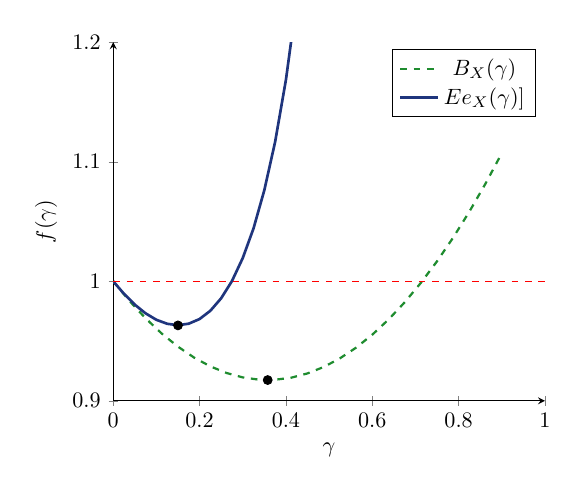
\begin{tikzpicture}[scale = 0.8]
        \begin{axis}[
            axis lines = left,
            xlabel = \(\gamma\),
            ylabel = {\(f(\gamma)\)},
            xmin=0, xmax=1,
            ymin=0.9, ymax=1.2
        ]
        \addplot[color=darkGreen,
            domain=0:0.9,
            dashed,
            line width=1pt
        ]{1 + (-0.4615) * x + (1.2901) / 2 * x * x};
        \addlegendentry{\(B_X(\gamma)\)}

        \addplot[color=darkBlue,
            domain=0:0.6,
            line width=1.2pt
        ]{-0.65/(x - 0.65) * exp(-2 * x)};
        \addlegendentry{\(Ee_X(\gamma)]\)}

        \addplot[color=black,mark=*] coordinates {(0.3578, 0.9174)};
        \addplot[color=black,mark=*] coordinates {(0.15, 0.9631)};
        \addplot[color=red,
            domain=0:3,
            dashed
        ]{1};
        \end{axis}
     \end{tikzpicture}
    \end{center}
    % \caption{Plot of the function $Ee_X(\gamma)$ with its bound $B_X(\gamma)$, where $X$ has probability density function $f(x) = 0.65 e^{-0.65(x + 2)}$.}
    % \label{fig:negativeDriftPic2}
\end{figure}

If $E[X] > 0$ then in some neighborhood around $\gamma = 0$ would be greater than any $e^{\frac{c \gamma^2}{2}}$. To proof it, consider function $G_c(\gamma) = e^{\frac{c \gamma^2}{2}}$, then

$$\frac{\partial G_c(\gamma)}{\partial \gamma} = c\gamma\ G_c(\gamma) = g(\gamma),$$

$g(0) = 0 < E[X]$ and $Ee_X(0) = B_X(0) = 1$. Hence both of requirements are not feasible.

\pagebreak

Example for $X \sim \mathcal{N}(1, 1)$:

\begin{figure}[h!]
    \begin{center}
     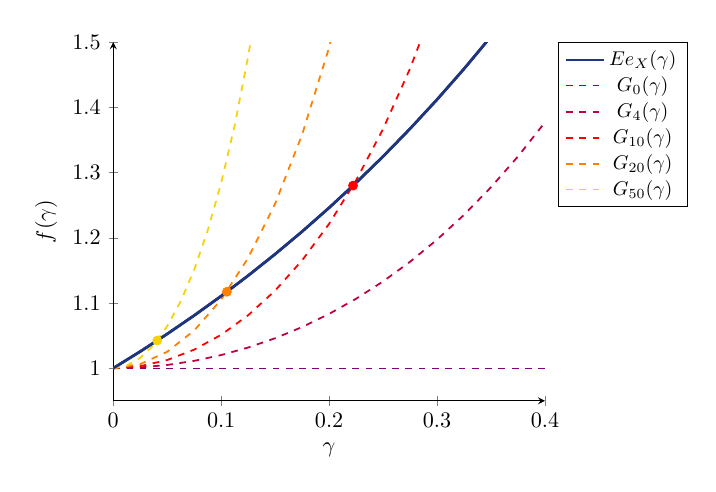
\begin{tikzpicture}[scale = 0.8]
        \begin{axis}[
            legend style=
            {nodes={scale=0.9, transform shape},
            at={(1.33,1)},anchor=north east},
            axis lines = left,
            xlabel = \(\gamma\),
            ylabel = {\(f(\gamma)\)},
            xmin=0, xmax=0.4,
            ymin=0.95, ymax=1.5
        ]
        
        \addplot[color=darkBlue,
            domain=0:0.6,
            line width=1.2pt
        ]{exp((x^2 + 2*x) / 2)};
        
        \addlegendentry{\(Ee_X(\gamma)\)}

        \addplot[color=violet,
            domain=0:3,
            dashed
        ]{1};

        \addlegendentry{\(G_0(\gamma)\)}

        \addplot[color=purple,
            domain=0:0.6,
            line width=0.8pt,
            dashed
        ]{exp((4 * x^2) / 2)};

        \addlegendentry{\(G_4(\gamma)\)}

        \addplot[color=red,
            domain=0:0.6,
            line width=0.8pt,
            dashed
        ]{exp((10 * x^2) / 2)};

        \addlegendentry{\(G_{10}(\gamma)\)}

        \addplot[color=orange,
            domain=0:0.6,
            line width=0.8pt,
            dashed
        ]{exp((20 * x^2) / 2)};

        \addlegendentry{\(G_{20}(\gamma)\)}

        \addplot[color=brightYellow,
            domain=0:0.3,
            line width=0.8pt,
            dashed
        ]{exp((50 * x^2) / 2)};

        \addlegendentry{\(G_{50}(\gamma)\)}

        \addplot[color=darkBlue,
            domain=0:0.6,
            line width=1.2pt
        ]{exp((x^2 + 2*x) / 2)};

        \addplot[color=brightYellow,mark=*] coordinates {(0.0408, 1.0425)};
        \addplot[color=orange,mark=*] coordinates {(0.1053, 1.1172)};
        \addplot[color=red,mark=*] coordinates {(0.2222, 1.2801)};
        
        \end{axis}
     \end{tikzpicture}
    \end{center}
\end{figure}

\subsection*{Conclusions}

In the case of $\textbf{\text{zero}}$ expectation we cannot always guarantee sub-gausality, which has been proved by the example of series of even functions $\expx{a}$.

In the case of $\textbf{\text{positive}}$ expectation both criteria are not feasible, and if it is $\textbf{\text{negative}}$, then both are feasible.

\subsection{Comparing results for processes with negative drifts}

Consider a process \( \{ X_n \}_{n \in \mathbb{N}}\) with negative drift (i.e. \(E[X_{t + 1} - X_{t} | X_t = s] < 0\) for all \(s\)) and special requirement for probability:

\[
    \Pr[X_{t + 1} - X_{t} = j] \leq \frac{r}{(1 + \varepsilon)^{j + s}},
\]

for some \(\varepsilon, r, s > 0\) and for all \(j \geq -s\).

Because this process has negative drift we need to impose restrictions for values of \(s\). Also because summation of probabilities for all possible values of \(X_{t + 1} - X_{t}\) must be equals 1 we need to find \(r\).

\begin{align*}
    \sum_{j = -s}^{+\infty} Pr[X_{t + 1} - X_t = j] &\leq \sum_{j = -s}^{+\infty} \frac{r}{(1 + \varepsilon)^{j + s}} = r \sum_{j = 0}^{+\infty} \frac{1}{(1 + \varepsilon)^{j}} \\
    1 &\leq r \frac{1}{1 - \frac{1}{1 + \varepsilon}} = r \frac{1 + \varepsilon}{\varepsilon} \\
    r &\geq \frac{\varepsilon}{1 + \varepsilon} 
\end{align*}

Consider \(\Delta_t = X_{t + 1} - X_{t}\), than compute \(E[\Delta_t]\):

\begin{align*}
    E[\Delta_t] &= \sum_{j = -s}^{+\infty} j Pr[\Delta_t = j] \leq \sum_{j = -s}^{+\infty} j \frac{r}{(1 + \varepsilon)^{j + s}} \leq \sum_{j = 0}^{+\infty} (j - s) \frac{\varepsilon}{(1 + \varepsilon)^{j + 1}} = \\
    &= \sum_{j = 0}^{+\infty} j \frac{\varepsilon}{(1 + \varepsilon)^{j + 1}} - s \sum_{j = 0}^{+\infty}\frac{\varepsilon}{(1 + \varepsilon)^{j + 1}} = \frac{1}{\varepsilon} - s
\end{align*}

Also compute \(E\left[e^{\gamma \Delta_t}\right]\) for all positive \(\gamma\):

\begin{align*}
    E[e^{\gamma \Delta_t}] &= \sum_{j = -s}^{+\infty} e^{\gamma j} \Pr[\Delta_t = j] \leq e^{-\gamma s} \sum_{j = 0}^{+\infty} e^{\gamma j} \frac{\varepsilon}{(1 + \varepsilon)^{j + 1}} = \\
    &= e^{-\gamma s} \frac{\varepsilon}{1 + \varepsilon} \sum_{j = 0}^{+\infty} \left(\frac{e^\gamma}{1 + \varepsilon}\right)^j = e^{-\gamma s} \frac{\varepsilon}{1 + \varepsilon} \frac{1}{(1 - \frac{e^\gamma}{1 + \varepsilon})} = \frac{\varepsilon e^{-\gamma s}}{(1 + \varepsilon) - e^\gamma} 
\end{align*}

Finding minimum of previous function can be useful, so lets find \(\gamma_0\) where \(\frac{\partial E[e^{\gamma \Delta_t}]}{\partial \gamma} = 0\):

\begin{align*}
    \frac{\partial E[e^{\gamma \Delta_t}]}{\partial \gamma} &= \frac{\partial }{\partial \gamma} \left(\frac{\varepsilon e^{-\gamma s}}{(1 + \varepsilon) - e^\gamma}\right) = \varepsilon \frac{-s e^{-\gamma s} (1 + \varepsilon - e^\gamma) - e^{-\gamma s}(-e^\gamma)}{(1 + \varepsilon - e^\gamma)^2} = \\
    &= \frac{-\varepsilon e^{-\gamma s}}{(1 + \varepsilon - e^\gamma)^2} (e^\gamma (s + 1) - s (1 + \varepsilon)) = 0
\end{align*}
\begin{align*}
    e^{\gamma_0} (s + 1) - s (1 + \varepsilon) = 0
\end{align*}
\begin{align*}
    \gamma_0 = \ln\left(\frac{s}{s + 1}(1 + \varepsilon)\right)
\end{align*}

Define some variables for next calculations:

\begin{itemize}
    \item \(\gamma_1\) - point where math expectation of exponent intersects 1:
    \begin{align*}
        E[e^{\gamma_1 \Delta_t}] = 1
    \end{align*}
    \item \(\delta_0\) - point where math expectation of exponent intersects sub-gaussian boundary:
    \begin{align*}
        E[e^{\delta_0 \Delta_t}] = e^{\frac{c}{2}\delta_0^2}
    \end{align*}
    Of course if \(c = 0\) then \(\delta_0 = \gamma_1\)
    \item \(\gamma_m\) - point where probability by negative drift reach minimum
    \begin{align*}
        \gamma_m = \argmin \left(\ \frac{d}{s} \cdot p(\gamma) \cdot e^{-\gamma d}\ \right),
    \end{align*}
    where \(d := \frac{b - a}{2}\)

    Because we want probability to be as small as possible, define \(p(\gamma) = \frac{1}{1 - E[e^{\gamma \Delta_t}]}\). Consider derivative of probability function to conclude about boundaries of \(\gamma_m\):
    
    \begin{align*}
        \der{}{\gamma} \left(\frac{d e^{-\gamma d}}{s} p \right)= \frac{d e^{-\gamma d}}{s} \left(p'_\gamma - dp\right) = \frac{d e^{-\gamma d}}{s (1 - E[e^{\gamma \Delta_t}])} \left(\frac{E'_\gamma [e^{\gamma \Delta_t}]}{1 - E[e^{\gamma \Delta_t}]} - d\right)
    \end{align*}

    For all \(\gamma \in (0, \gamma_0)\) we have: \(\expp{\gamma} \in (0, 1)\) and \(E'_\gamma[e^{\gamma \Delta_t}] < 0\), hence derivative of probability is negative for all \(d\). After it for all \(\gamma \in [\gamma_0, \gamma_1)\) we have same limits for \(\expp{\gamma}\) and, because \(E'_\gamma[e^{\gamma \Delta_t}] \geq 0\), it grows to 1, hence somewhere between \(\gamma_0\) and \(\gamma_1\) derivative becomes 0, hence
    
    \begin{align*}
        \gamma_m \in [\gamma_0, \gamma_1)
    \end{align*}

    Obvious that \(\lim\limits_{d \to +\infty} \gamma_m = \gamma_1\).

    \item \(c_m\) - value of parameter \(c\) when \(\delta_0 = \frac{s}{c}\)
    
    We can calculate it from definition of \(\delta_0\):

    \begin{gather*}
        E[e^{\delta_0 \Delta_t}] = e^{\frac{c}{2}\delta_0^2} \\
        \frac{\varepsilon e^{-\frac{s^2}{c_m}}}{(1 + \varepsilon) - e^{\frac{s}{c_m}}}  = e^{\frac{s^2}{2c_m}} \\
        \varepsilon = ((1 + \varepsilon) - e^{\frac{s}{c_m}}) e^{\frac{3s^2}{2c_m}}
    \end{gather*}

    We know that \(e^{\frac{s}{c_m}} \in [1, 1 + \varepsilon)\), so let us denote \(\delta = e^{\frac{s}{c_m}} - 1\)

    \begin{gather*}
        \varepsilon = (1 + \varepsilon - 1 - \delta) (1 + \delta)^{\frac{3s}{2}} \\
        \frac{e}{e - \delta} = (1 + \delta)^{\frac{3s}{2}} \\
        1 + \frac{\delta}{\varepsilon - \delta} = (1 + \delta)^{\frac{3s}{2}}
    \end{gather*}

    Let us denote \(\alpha = \frac{3s}{2}\). By using Taylor series we have \((1 + \delta)^{\alpha} \geq 1 + \alpha \delta + \frac{\alpha (\alpha - 1)}{2} \delta^2\)

    \begin{gather*}
        1 + \frac{\delta}{\varepsilon - \delta} \geq 1 + \alpha \delta + \frac{\alpha (\alpha - 1)}{2} \delta^2 \\
        \frac{1}{\varepsilon - \delta} \geq \alpha + \frac{\alpha (\alpha - 1)}{2} \delta \\
        \frac{1}{\alpha} \geq \delta^2 \left(-\frac{\alpha - 1}{2}\right) + \delta \left(\frac{\alpha - 1}{2}\varepsilon - 1\right) + \varepsilon \\
        \delta^2\left(\frac{\alpha - 1}{2}\right) + \delta \left(1 - \frac{\alpha - 1}{2}\varepsilon\right) + \left(\frac{1}{\alpha} - \varepsilon\right) \geq 0 \\
        \delta \approxeq \frac{\frac{\alpha - 1}{2}\varepsilon - 1 + \sqrt{\left(1 - \frac{\alpha - 1}{2}\varepsilon\right)^2 - 2 (\alpha - 1)(\frac{1}{\alpha} - \varepsilon)}}{\alpha - 1} \\
        \delta \approxeq \frac{\varepsilon}{2} - \frac{1}{\alpha - 1} + \sqrt{\left(\frac{\varepsilon}{2} - \frac{1}{\alpha - 1}\right)^2 + 2 \frac{\alpha \varepsilon - 1}{\alpha(\alpha - 1)}} \\
        \delta \approxeq \frac{\varepsilon}{2} - \frac{1}{\alpha - 1} + \sqrt{\left(\frac{\varepsilon}{2} + \frac{1}{\alpha - 1}\right)^2 - \frac{2}{\alpha^2(\alpha - 1)}} \\
        \delta \approxeq \varepsilon - \frac{2}{\alpha^2(\varepsilon(\alpha - 1) + 2)}
    \end{gather*}

    Then we have approximation:

    \begin{gather*}
        c_m \approxeq \frac{s}{\ln\left(1 + \varepsilon - \frac{2}{\alpha^2(\varepsilon(\alpha - 1) + 2)}\right)}
    \end{gather*}
    
    or 

    \begin{gather*}
        c_m \approxeq \frac{s}{\ln\left(1 + \frac{\varepsilon}{2} - \frac{1}{\alpha - 1} + \sqrt{\left(\frac{\varepsilon}{2} + \frac{1}{\alpha - 1}\right)^2 - \frac{2}{\alpha^2(\alpha - 1)}}\right)}
    \end{gather*}

    Second approximation is better, but first is better in demonstration of behavior of 
    \(c_m\) regarding \(s\) and \(\varepsilon\).

    By why we have \(c_m\) and what it give us? Significance of it is that if we consider probability by sub-gaussian theorem:

    \begin{align*}
        \Pr \left[T \leq \frac{d}{\varepsilon}\right] \leq e^{- \frac{d}{2} \min\left(\delta_0, \frac{s}{c}\right)},
    \end{align*}

    if \(c = c_m\) then probability will take the smallest values over values of positive \(c\), because if \(c\) grows then \(\frac{s}{c}\) decreases, but \(\delta_0\) increases since \( e^{\frac{c}{2} \gamma^2}\) grows over \(c\) too.

    \item \(N(d)\) - function of probability for \(d:= \frac{b - a}{2}\) given by negative drift theorem, hence:
    
    \begin{align*}
        N(d) = \frac{d p(\gamma_m)}{s}  e^{-\gamma_m d}
    \end{align*}

    \item \(G(d)\) - function of probability for \(d:= \frac{b - a}{2}\) given by theorem for sub-gaussian processes, hence:
    
    \begin{align*}
        G(d) = \exp \left(-\frac{d s}{2 c_m}\right)
    \end{align*}
\end{itemize}

Consider \(p(\gamma_m)\) in \(N(d)\). By definition of \(\gamma_m\),  \(p(\gamma_m)\) - function over \(d\). We want to find asymptotic behavior regarding \(d\) of it.

Because \(\gamma_m\) - is a point where original probability reaches minimum over \(\gamma\) we have from derivative of probability:

\begin{gather*}
    \left(\frac{E'_\gamma [e^{\gamma_m \Delta_t}]}{1 - E[e^{\gamma_m \Delta_t}]} - d\right) = 0 \\
    E'_\gamma [e^{\gamma_m \Delta_t}] p(\gamma_m) = d \\
    p(\gamma_m) = \frac{d}{E'_\gamma [e^{\gamma_m \Delta_t}]}
\end{gather*}

We know, that if \(d \to +\infty\) then \(\gamma_m \to 1\), hence \(\lim\limits_{d \to +\infty} \frac{p(\gamma_m)}{d} = \lim\limits_{d \to +\infty} \frac{1}{E'_\gamma [e^{\gamma_m \Delta_t}]} = \frac{1}{E'_\gamma [e^{\gamma_1 \Delta_t}]} \). And because \(\gamma_1\) is independent from \(d\), we conclude:

\begin{align*}
    p(\gamma_m) = \mathcal{O} (d)
\end{align*}

Then we want to consider such ratio:

\begin{align*}
    \limd \frac{\ln(N(d))}{\ln(G(d))}
\end{align*}

Compute it:

\begin{align*}
    \limd \frac{\ln(N(d))}{\ln(G(d))} &= \limd \frac{\ln(\frac{d p(\gamma_m)}{s}  e^{-\gamma_m d})}{-\frac{d s}{2 c_m}} = \limd \frac{\ln(d) - \ln(s) + \ln(p(\gamma_m)) - \gamma_m d}{\frac{- d s}{2 c_m}} = \\
    &= \limd \frac{\ln(\mathcal{O}(\gamma_m)) - \gamma_m d}{\frac{- d s}{2 c_m}} = \limd \frac{\gamma_m d}{\frac{d s}{2 c_m}} = \limd \frac{2 c_m \gamma_m}{s} = \frac{2 \gamma_1 c_m}{s} = \frac{2 \gamma_1}{\delta_0^m}
\end{align*}

Where \(\delta_0^m = \delta_0(c_m)\).

Obvious that \(\frac{\gamma_1}{\delta_0^m} \leq 1\) since by definition \(\delta_0^m \geq \gamma_1\). But is true that \(\frac{\gamma_1}{\delta_0^m} \geq \frac{1}{2}\) ?

Consider situation when math expectation in near zero. Then \(\gamma_0 \to 0\) and in some neighborhood of zero sub-gaussian boundary and expectation of exponent will behave as quadratic functions.

In this case denote: 

\begin{align*}
    E[e^{\gamma \Delta_t}] \approxeq 1 + e_1 \gamma + \frac{e_2}{2} \gamma^2,
\end{align*}

where \(e_1 = E[\Delta_t],\ e_2 = E[\Delta_t^2]\).

And:

\begin{align*}
    e^{\frac{c \gamma^2}{2}} \approxeq 1 + \frac{c \gamma^2}{2}
\end{align*}

Then:

\begin{gather*}
    \gamma_1 = -\frac{2e_1}{e_2} \\
    \delta_0 = -\frac{2e_1}{e_2 - c}
\end{gather*}

But we must best \(\delta_0\), so we must find \(c_m\):

\begin{gather*}
    \delta_0^m = \frac{s}{c_m} \\
    -\frac{2e_1}{e_2 -c_m} = \frac{s}{c_m} \\
    c_m = \frac{s e_2}{s - 2e_1}
\end{gather*}

Then:

\begin{gather*} 
    \delta_0^m = \frac{2e_1}{e_2 - c_m} \\
    \delta_0^m = \frac{s - 2e_1}{e_2}
\end{gather*}

Ratio will be: 

\begin{gather*}
    \frac{2 \gamma_1}{\delta_0^m} = 2 - \frac{2 s}{s - 2 e_1} \to 0
\end{gather*}

We conclude that value of this ratio depends from \(s \text{ and } \varepsilon\) and with conditions it is greater than 1 and with another it is less than 1.

\begin{exmp}
    If \(s \to +\infty\) then \(\gamma_0 \to \ln(1 + \varepsilon)\). Because \(\gamma_0 \leq \gamma_1\) hence \(\gamma_1 \to \ln(1 + \varepsilon)\). 
    
    Consider \(\frac{c_m}{s}\):

    \begin{align*}
        \lim\limits_{s \to +\infty} \frac{c_m}{s} = \lim\limits_{s \to +\infty} \frac{\frac{s}{\ln\left(1 + \varepsilon - \frac{2}{\alpha^2(\varepsilon(\alpha - 1) + 2)}\right)}}{s} = \frac{1}{\ln(1 + \varepsilon)}
    \end{align*}

    Then:

    \begin{align*}
        \limd \frac{\ln(N(d))}{\ln(G(d))} = 2 > 1
    \end{align*}
\end{exmp}

\begin{exmp}

    If \(s \to \frac{1}{\varepsilon}\) then \(\gamma_0, \gamma_1 \to 0\), but \(\delta_0^m\) decreases not so fast.

    If we take \(s = 0.54, \varepsilon = 2\), then \(
        \delta_0^m \approxeq 0.55, \gamma_1 \approxeq 0.13\) and then:

    \begin{align*}
        \limd \frac{\ln(N(d))}{\ln(G(d))} \approxeq 0.473 < 1
    \end{align*}

\end{exmp}





\section{Tail bounds}
\subsection{Upper bounds}
Consider a process $\{X_t\}_{t \in \mathbb{N}}$ with positive drift (i.e. $E[X_{t + 1} - X_t |\ X_t = s] \geq 0$ for all $s$) and another process $\{Y_t\}_{t \in \mathbb{N}}$ such that $Y_t = X_t - \varepsilon t$ and it has negative drift (i.e. $E[Y_{t + 1} - Y_t |\ Y_t = s] \leq 0$ for all $s$).

Our aim is to bound the probability $\Pr[T_X \leq t_0]$, where $T_X$ is the first time when $X_t \geq b$ for some $b > X_0$ and for $t_0$. We first note that

\begin{align*}
    \Pr[T_X \leq t_0] \leq \Pr[X_{t_0} \geq b] \leq \Pr[Y_{t_0} \geq b - \varepsilon t_0].
\end{align*}

Since $\{Y_t\}_{t \in \mathbb{N}}$ is a process with negative drift, it is a subject to Theorem \cite{}. Hence, we have

\begin{align*}
    \Pr[Y_{t_0} \geq b - \varepsilon t_0] \leq t_0 D p e^{-\gamma(b - \varepsilon t_0 - a)},
\end{align*}

which also implies

\begin{align*}
    \Pr[T_X \leq t_0] \leq t_0 D p e^{-\gamma(b - \varepsilon t_0 - a)}.
\end{align*}

Let $t_0 := \frac{\kappa (b - a)}{\varepsilon}$. Then we compute
\begin{align*}
    \Pr\left[T_X \leq \frac{\kappa (b - a)}{\varepsilon}\right] \leq \frac{\kappa (b - a)}{\varepsilon} D p e^{-\gamma(1 - \kappa)(b - a)}.
\end{align*}

For example we can use $\kappa = \frac{1}{2}$ and obtain

\begin{align*}
    \Pr\left[T_X \leq \frac{(b - a)}{2\varepsilon}\right] \leq \frac{(b - a)}{2\varepsilon} D p e^{-\gamma\frac{(b - a)}{2}}.
\end{align*}

\subsection{Lower bounds}

Consider a process $\{X_t\}_{t \in \mathbb{N}}$ with positive drift (i.e. $E[X_{t + 1} - X_t |\ X_t = s] \geq 0$ for all $s$) and another process $\{Y_t\}_{t \in \mathbb{N}}$ such that $Y_t = \varepsilon t - X_t$ and it has negative drift (i.e. $E[Y_{t + 1} - Y_t |\ Y_t = s] \leq 0$ for all $s$).

Our aim is to bound the probability $\Pr[T_X > t_0]$, where $T_X$ is the first time when $X_t \geq b$ for some $b > X_0$ and for $t_0$. We first note that

\begin{align*}
    \Pr[T_X > t_0] \leq \Pr[X_{t_0} < b] \leq \Pr[Y_{t_0} > \varepsilon t_0 - b].
\end{align*}

Since $\{Y_t\}_{t \in \mathbb{N}}$ is a process with negative drift, it is a subject to Theorem \cite{}. Hence, we have

\begin{align*}
    \Pr[Y_t > \varepsilon t_0 - b] \leq t_0 D p e^{-\gamma(\varepsilon t_0 - b + a)},
\end{align*}

which also implies

\begin{align*}
    \Pr[T_X > t_0] \leq t_0 D p e^{-\gamma(\varepsilon t_0 - b + a)}.
\end{align*}

Let $t_0 := \frac{\kappa (b - a)}{\varepsilon}$. Then we compute
\begin{align*}
    \Pr\left[T_X > \frac{\kappa (b - a)}{\varepsilon}\right] \leq \frac{\kappa (b - a)}{\varepsilon} D p e^{-\gamma(\kappa - 1)(b - a)}.
\end{align*}

For example we can use $\kappa = \frac{3}{2}$ and obtain

\begin{align*}
    \Pr\left[T_X > \frac{3 (b - a)}{2\varepsilon}\right] \leq \frac{3(b - a)}{2\varepsilon} D p e^{-\gamma\frac{(b - a)}{2}}.
\end{align*}

% Lets take a look on process $\{X_t\}$ and its derivative process $\{Y_t\}$, where $Y_t = \varepsilon t - X_t$ and it has negative drift.

% Then we want to bounds $\Pr[T_X > t_0]$, where $T_X$ - first time $X_t \geq b$. 

% \begin{align*}
%     \Pr[T_X > t_0] \leq \Pr[X_{t_0} < b] \leq \Pr[Y_{t_0} > \varepsilon t_0 - b]
% \end{align*}

% Then, because $\{Y_t\}$ - process with negative drift, we may use the corresponding theorem *label*:

% \begin{align*}
%     \Pr[Y_t > \varepsilon t_0 - b] \leq t_0 D p e^{-\gamma(\epsilon t_0 - b + a)}
% \end{align*}

% Lets rewrite some to $T_X$: 

% \begin{align*}
%     \Pr[T_X > t_0] \leq t_0 D p e^{-\gamma(\epsilon t_0 - b + a)}
% \end{align*}

% Replace $t_0$ with another expression:

% \begin{align*}
%     t_0 := \frac{\kappa (b - a)}{\varepsilon}
% \end{align*}

% And then:

% \begin{align*}
%     \Pr\left[T_X > \frac{\kappa (b - a)}{\varepsilon}\right] \leq \frac{\kappa (b - a)}{\varepsilon} D p e^{-\gamma(\kappa - 1)(b - a)}
% \end{align*}

% For example use $\kappa = \frac{3}{2}$:

% \begin{align*}
%     \Pr\left[T_X > \frac{3 (b - a)}{2\varepsilon}\right] \leq \frac{3(b - a)}{2\varepsilon} D p e^{-\gamma\frac{(b - a)}{2}}
% \end{align*}

% ПОВТОРИТЬ ЕЩЕ РАЗ ПРЕДЫДУЩИЙ ПАРАГРАФ

\section{Time bounds for process with variable $\lambda$}
\cm
\subsection{Case when $\lambda$ is a random variable}
Consider the total progress $\Delta X$ made in $T$ iterations. It is a sum of all progresses $\Delta X_i$ made in each of $T$ iterations.
\[
    \Delta X = \sum_{i = 0}^{T} \Delta X_i
\]

By Wald's equality we have

\[
    E[\Delta X] = E\left[\sum_{i = 1}^{T} \Delta X_i\right].
\]

If we assume that $E[\Delta X_i]$ is a constant or at least we can give relatively sharp lower and upper bounds on it, then
\[
    E[\Delta X] = E\left[\sum_{i = 1}^{T} \Delta X_i\right] \thickapprox E[T] E[\Delta X_i].
\]

Let $\Lambda$ be the total cost, which is the total number of fitness evaluations (the fitness evaluations in iteration $i$ equals $\lambda_i$). Since $\lambda$ is a random variable, each $\lambda_i$ has the same expectation. Therefore, we have
\[
    E\left[\Lambda\right] = E\left[\sum_{i = 1}^{T} \lambda_i\right] = E[T] E[\lambda] \thickapprox \frac{E[\Delta X] E[\lambda]}{E[\Delta X_i]}
\]

If we denote $\vartheta_\lambda = \frac{E[\Delta X_i]}{E[\lambda]}$, which is the expected progress per fitness evaluation, then the previous equation is simplified to
\[
    E[\Lambda] \thickapprox \frac{E[\Delta X]}{\vartheta_\lambda}.
\]
% $\vartheta_{\lambda, X_t} = \nu (\lambda, X_t)$

\section{Conclusion}
\cm


\bibliographystyle{alpha}
\bibliography{bibliography}

\end{document}